% Hatsune Miku Theme - LaTeX Showcase
% No color screams. Every color sings.

\documentclass[12pt, a4paper]{article}

% =============================================================================
% Packages
% =============================================================================

\usepackage[utf8]{inputenc}
\usepackage[T1]{fontenc}
\usepackage[english]{babel}
\usepackage{amsmath, amssymb, amsthm}
\usepackage{graphicx}
\usepackage{xcolor}
\usepackage{hyperref}
\usepackage{listings}
\usepackage{booktabs}
\usepackage{geometry}
\usepackage{fancyhdr}
\usepackage{tikz}
\usepackage{algorithm}
\usepackage{algpseudocode}

% =============================================================================
% Document Setup
% =============================================================================

\geometry{margin=1in}

% Define Miku colors
\definecolor{mikuteal}{HTML}{39C5BB}
\definecolor{mikupink}{HTML}{E05096}
\definecolor{mikubg}{HTML}{1A1F24}
\definecolor{mikufg}{HTML}{C8DCD9}

% Hyperref setup
\hypersetup{
    colorlinks=true,
    linkcolor=mikuteal,
    urlcolor=mikuteal,
    citecolor=mikupink
}

% Code listing setup
\lstset{
    basicstyle=\ttfamily\small,
    keywordstyle=\color{mikuteal}\bfseries,
    commentstyle=\color{gray}\itshape,
    stringstyle=\color{mikupink},
    numbers=left,
    numberstyle=\tiny\color{gray},
    breaklines=true,
    frame=single,
    backgroundcolor=\color{mikubg!10}
}

% Header/Footer
\pagestyle{fancy}
\fancyhf{}
\fancyhead[L]{\textcolor{mikuteal}{Miku Stage}}
\fancyhead[R]{\thepage}
\fancyfoot[C]{\textcolor{gray}{Hatsune Miku Theme}}

% Custom commands
\newcommand{\miku}{\textcolor{mikuteal}{Miku}}
\newcommand{\highlight}[1]{\textcolor{mikupink}{\textbf{#1}}}
\newcommand{\code}[1]{\texttt{#1}}

% Theorem environments
\newtheorem{theorem}{Theorem}[section]
\newtheorem{lemma}[theorem]{Lemma}
\newtheorem{definition}{Definition}[section]

% =============================================================================
% Document Content
% =============================================================================

\title{\textcolor{mikuteal}{Hatsune Miku Theme} \\
       \large No Color Screams, Every Color Sings}
\author{Miku Fan}
\date{\today}

\begin{document}

\maketitle

\begin{abstract}
This document showcases \LaTeX{} syntax highlighting for the Hatsune Miku VS Code theme.
It demonstrates various \LaTeX{} features including math equations, code listings,
tables, figures, and custom formatting with \miku{} colors.
\end{abstract}

\tableofcontents
\newpage

% =============================================================================
% Sections and Text
% =============================================================================

\section{Introduction}
\label{sec:intro}

Welcome to the \highlight{Miku Stage}! This document demonstrates \LaTeX{} features
for the Hatsune Miku theme. See Section~\ref{sec:math} for mathematical content.

\subsection{Text Formatting}

\LaTeX{} supports various text formatting options:
\begin{itemize}
    \item \textbf{Bold text} for emphasis
    \item \textit{Italic text} for titles
    \item \texttt{Monospace} for code
    \item \textsc{Small Caps} for headers
    \item \underline{Underlined} for highlights
\end{itemize}

\paragraph{Paragraph Heading}
This is a paragraph with a heading. The canonical Miku color is \textcolor{mikuteal}{\#39C5BB}.

\subparagraph{Subparagraph}
Even deeper nesting is possible.

% =============================================================================
% Mathematics
% =============================================================================

\section{Mathematical Expressions}
\label{sec:math}

\subsection{Inline and Display Math}

Inline math: The frequency $f = \frac{1}{T}$ where $T$ is the period.

Display math:
\[
    E = mc^2
\]

Numbered equation:
\begin{equation}
    \label{eq:fourier}
    F(\omega) = \int_{-\infty}^{\infty} f(t) e^{-i\omega t} \, dt
\end{equation}

Reference to Equation~\eqref{eq:fourier}.

\subsection{Complex Equations}

Multi-line alignment:
\begin{align}
    \nabla \cdot \mathbf{E} &= \frac{\rho}{\varepsilon_0} \\
    \nabla \cdot \mathbf{B} &= 0 \\
    \nabla \times \mathbf{E} &= -\frac{\partial \mathbf{B}}{\partial t} \\
    \nabla \times \mathbf{B} &= \mu_0 \mathbf{J} + \mu_0 \varepsilon_0 \frac{\partial \mathbf{E}}{\partial t}
\end{align}

Matrix:
\[
    \mathbf{A} = \begin{pmatrix}
        a_{11} & a_{12} & a_{13} \\
        a_{21} & a_{22} & a_{23} \\
        a_{31} & a_{32} & a_{33}
    \end{pmatrix}
\]

Cases:
\[
    |x| = \begin{cases}
        x & \text{if } x \geq 0 \\
        -x & \text{if } x < 0
    \end{cases}
\]

\subsection{Theorems and Proofs}

\begin{definition}
A \emph{virtual singer} is a synthesized voice capable of producing musical performances.
\end{definition}

\begin{theorem}[Miku's Energy Theorem]
\label{thm:energy}
For any performance $P$ with duration $t$ and BPM $b$, the energy consumed $E$ satisfies:
\[
    E = k \cdot t \cdot \sqrt{b}
\]
where $k$ is a constant depending on the voice bank.
\end{theorem}

\begin{proof}
By induction on the number of beats. The base case $n=1$ is trivial.
Assume the result holds for $n$ beats. For $n+1$ beats:
\[
    E_{n+1} = E_n + \Delta E = k \cdot t_n \cdot \sqrt{b} + k \cdot \Delta t \cdot \sqrt{b}
\]
which completes the proof.
\end{proof}

\begin{lemma}
The energy function is monotonically increasing.
\end{lemma}

% =============================================================================
% Code Listings
% =============================================================================

\section{Code Examples}

\subsection{Python Code}

\begin{lstlisting}[language=Python, caption={Miku Synthesizer Class}]
class DigitalDiva:
    """Virtual Singer implementation."""

    CANONICAL_COLOR = "#39C5BB"

    def __init__(self, name="Hatsune Miku"):
        self.name = name
        self._energy = 100

    def sing(self, song: str) -> str:
        if self._energy < 10:
            raise ValueError("Low energy")
        self._energy -= 10
        return f"[MIKU] Now singing: {song}"
\end{lstlisting}

\subsection{JavaScript Code}

\begin{lstlisting}[language=JavaScript, caption={Performance Function}]
async function perform(song, bpm = 120) {
    console.log(`Playing: ${song} at ${bpm} BPM`);
    await new Promise(r => setTimeout(r, 1000));
    return { song, bpm, status: 'complete' };
}
\end{lstlisting}

% =============================================================================
% Tables
% =============================================================================

\section{Tables}

\begin{table}[htbp]
    \centering
    \caption{Miku Voice Bank Versions}
    \label{tab:versions}
    \begin{tabular}{@{} lccc @{}}
        \toprule
        \textbf{Version} & \textbf{Year} & \textbf{Engine} & \textbf{Color} \\
        \midrule
        V2 Classic & 2007 & VOCALOID2 & \textcolor{mikuteal}{\#39C5BB} \\
        Append     & 2010 & VOCALOID2 & Various \\
        V3         & 2013 & VOCALOID3 & \textcolor{mikuteal}{\#39C5BB} \\
        V4X        & 2016 & VOCALOID4 & \textcolor{mikuteal}{\#39C5BB} \\
        NT         & 2020 & Piapro    & \#00BCD4 \\
        \bottomrule
    \end{tabular}
\end{table}

% =============================================================================
% Figures and TikZ
% =============================================================================

\section{Graphics}

\subsection{TikZ Diagram}

\begin{figure}[htbp]
    \centering
    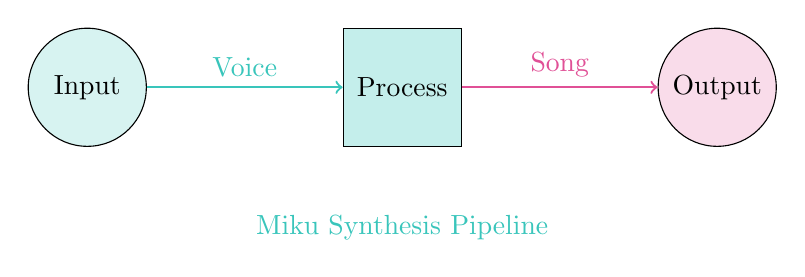
\begin{tikzpicture}
        % Nodes
        \node[draw, circle, fill=mikuteal!20, minimum size=1.5cm] (input) at (0,0) {Input};
        \node[draw, rectangle, fill=mikuteal!30, minimum size=1.5cm] (process) at (4,0) {Process};
        \node[draw, circle, fill=mikupink!20, minimum size=1.5cm] (output) at (8,0) {Output};

        % Arrows
        \draw[->, thick, mikuteal] (input) -- node[above] {Voice} (process);
        \draw[->, thick, mikupink] (process) -- node[above] {Song} (output);

        % Label
        \node[below=0.5cm] at (4,-1) {\textcolor{mikuteal}{Miku Synthesis Pipeline}};
    \end{tikzpicture}
    \caption{Voice synthesis pipeline diagram}
    \label{fig:pipeline}
\end{figure}

% =============================================================================
% Algorithms
% =============================================================================

\section{Algorithms}

\begin{algorithm}
\caption{Performance Optimization}
\label{alg:perform}
\begin{algorithmic}[1]
\Require Song list $S$, Energy $E$, BPM $b$
\Ensure Optimized performance order
\State $result \gets []$
\For{$song \in S$}
    \If{$E \geq 10$}
        \State $E \gets E - 10$
        \State $result.\text{append}(song)$
    \Else
        \State \textbf{break}
    \EndIf
\EndFor
\State \Return $result$
\end{algorithmic}
\end{algorithm}

% =============================================================================
% Bibliography
% =============================================================================

\section{References}

\begin{thebibliography}{9}
    \bibitem{vocaloid}
    Crypton Future Media,
    \textit{Hatsune Miku: The Virtual Singer},
    2007.

    \bibitem{synthesis}
    H. Kenmochi,
    ``Singing synthesis system VOCALOID,''
    \textit{Proc. ICMC}, 2007.
\end{thebibliography}

% =============================================================================
% Appendix
% =============================================================================

\appendix
\section{Color Reference}

\begin{center}
\begin{tabular}{ll}
    \textcolor{mikuteal}{\rule{1cm}{1cm}} & \code{\#39C5BB} - Miku Teal \\
    \textcolor{mikupink}{\rule{1cm}{1cm}} & \code{\#E05096} - Magenta LED \\
\end{tabular}
\end{center}

\end{document}
